\documentclass[oneside,10pt,a4paper]{article}

\title{Performance Analysis of OpenFlow Hardware\\[0.3cm]
\Large{}}
\author{Michiel Appelman \and Maikel de Boer}

% (c) 2014 Michiel Appelman
%Packages
\usepackage[english]{babel}
\usepackage{verbatim} 
\usepackage{longtable}        %tables over meerdere pagina's
\usepackage{fancyhdr}         %Fancy headers
\usepackage{pdfpages}         %Includen van pdf's
\usepackage[toc,page]{appendix}         %Bijlagen
\usepackage{url}        %Mooie url's
\usepackage{xspace}         %Spatie na commando
\usepackage{color}        %text kleuren
\usepackage{graphicx}         %plaatjes includen
\usepackage{fancyvrb}     %extra verbatime (size) mogelijkheden
\usepackage{multicol}     %multicolumn
\usepackage{listings}
\usepackage{textcomp}
\usepackage{subcaption}
\usepackage{setspace}
\usepackage{palatino}
\usepackage{geometry}
\usepackage{eurosym}
\usepackage{bytefield}
\usepackage{hyperref}
\usepackage{fixltx2e}
\usepackage{xcolor}
\usepackage{colortbl}
\usepackage{float}
\usepackage{paralist}
\usepackage[printonlyused]{acronym}
\usepackage[T1]{fontenc}
%%

%% You want it in Sans Serif Helvetica?
%\usepackage[scaled]{helvet}
%\renewcommand*\familydefault{\sfdefault}

\newcommand{\HRule}{\hspace*{\fill}\rule{0.6\linewidth}{0.2mm}\hspace*{\fill}}
\newcommand{\acrstyle}[1]{\uppercase{#1}}
\newcommand{\expstyle}[1]{#1}

%highlighting in listings 
\definecolor{light-gray}{gray}{0.60}
\definecolor{light}{gray}{0.80}


\addtolength{\oddsidemargin}{-10mm}
\addtolength{\evensidemargin}{-10mm}
\addtolength{\textwidth}{20mm}
\textheight = 53\baselineskip
\advance\textheight by \topskip

% Table of Contents Depth
\setcounter{tocdepth}{2}

% Dutch style of paragraph formatting, i.e. no indents. 
\setlength{\parskip}{1.3ex plus 0.2ex minus 0.2ex}
\setlength{\parindent}{0pt}

%%Hyperref
\hypersetup{
    unicode=false,          % non-Latin characters in Acrobat’s bookmarks
    pdftoolbar=true,        % show Acrobat’s toolbar?
    pdfmenubar=true,        % show Acrobat’s menu?
    pdffitwindow=false,     % window fit to page when opened
    pdfstartview={FitH},    % fits the width of the page to the window
    pdftitle={Performance Analysis of OpenFlow Hardware},    % title
    pdfauthor={Michiel Appelman and Maikel de Boer},     % author
    pdfsubject={OpenFlow},   % subject of the document
    pdfkeywords={openflows,hardware,performance,sdn,onf,flowvisor}, % list of keywords
    pdfnewwindow=true,      % links in new window
    colorlinks=true,       % false: boxed links; true: colored links
    linkcolor=black,          % color of internal links
    citecolor=black,        % color of links to bibliography
    filecolor=magenta,      % color of file links
    urlcolor=blue           % color of external links
%    linkcolor=black,          % color of internal links
%    citecolor=black,        % color of links to bibliography
%    filecolor=black,      % color of file links
%    urlcolor=black           % color of external links
}

% Line break after paragraph title
\makeatletter
\renewcommand\paragraph{\@startsection{paragraph}{4}{\z@}%
  {-2.25ex\@plus -1ex \@minus -.2ex}%
  {.2ex \@plus .2ex}%
  {\normalfont\normalsize\bfseries}}
\makeatother

% Less hspacing at subsubsection
\makeatletter
\renewcommand\subsubsection{\@startsection{subsubsection}{3}{\z@}%
  {-2.25ex\@plus -1ex \@minus -.2ex}%
  {.2ex \@plus .2ex}%
  {\normalfont\normalsize\bfseries}}
\makeatother

\makeatletter
\def\console{%
  \color{white}\ttfamily\footnotesize
  \def\verbatim@processline{%
    {\setbox0=\hbox{\the\verbatim@line}%
    \hsize=\wd0 \the\verbatim@line\par}}%
  \@minipagetrue
  \@tempswatrue
  \@totalleftmargin\z@
  \setbox0=\vbox\bgroup \verbatim
}
\def\endconsole{%
  \endverbatim
  \unskip\setbox0=\lastbox
  \egroup
  \colorbox{black}{\box0}%
}
\makeatother

\hyphenation{Net-FPGA}

\begin{document}
	\pagenumbering{roman}
	% (c) 2014 Michiel Appelman
%\begin{titlepage}
%	\begin{center}
%		
%		\hfill \\[2.4cm]
%		
\includegraphics[width=8cm]{./includes/uva.pdf}\\[2cm]
%		\HRule\\[2cm]
%		{\huge \bfseries Performance Analysis of OpenFlow Hardware}\\[8cm]
%		
%		\vfill
%		
%		Michiel Appelman\\[0.3cm]
%		Maikel de Boer\\[0.6cm]
%		2012
%	\end{center}
%\end{titlepage}

\clearpage
\begin{titlepage}
	\begin{center}
		\hfill \\[2cm]
		
\includegraphics[width=8cm]{./includes/uva.pdf}\\[0.4cm]
		{\Large \textsc{MSc Systems \&{} Network Engineering}}\\[4.5cm]
		
		% Title
		\HRule \\[0.6cm]
		{ \huge \bfseries Architecture of a dynamic VPN in OpenFlow}\\[0.4cm]
		\HRule \\[4.2cm]
		%
\includegraphics[width=7cm]{./includes/uva.pdf}\\[0.2cm]
		%\rule{\linewidth}{0.2mm} \\[0.5cm]
		% Author and supervisor
		\begin{minipage}
			{0.4
			\textwidth} 
			\begin{flushleft}
				\large \emph{By:}\\
				Michiel \textsc{Appelman} \\
				{\footnotesize \texttt{michiel.appelman@os3.nl}}
			\end{flushleft}
		\end{minipage}
		\begin{minipage}
			{0.4
			\textwidth} 
			\begin{flushright}
				\large \emph{Supervisor:} \\
				Rudolf \textsc{Strijkers} \\
				{\footnotesize \texttt{rudolf.strijkers@tno.nl}}
				\hfill
			\end{flushright}
		\end{minipage}
		
		\hfill \\[4cm]
		
		% Bottom of the page
		{\large \today}
	\end{center}
\end{titlepage}

\cleardoublepage 

	
	% (c) 2014 Michiel Appelman
\vspace*{\fill}
{\section*{Summary}\addcontentsline{toc}{section}{Summary}
\label{sec:summary}

Hello world.

% section summary (end)
}
\vspace*{\fill}
	\clearpage

	% Reset acronyms.
	\acresetall
	\setlength{\parskip}{0ex plus 0.5ex minus 0.2ex}
	
	\tableofcontents
	\clearpage

	\listoffigures
	\listoftables
	\clearpage
	
	% Reset acronyms.
	\acresetall
	%%%%%%%%%%%%%%%%%%%%%%%%%%%
	%%%%%%%%%%%%%%%%%%%%%%%%%%%
		\pagenumbering{arabic}
		% Dutch style of paragraph formatting, i.e. no indents.
		\setlength{\parskip}{1.3ex plus 0.2ex minus 0.2ex}
		\pagestyle{fancy}
		\renewcommand{\sectionmark}[1]{% 
		\markboth{#1}{}}
		\fancyhead[L]{\small{\nouppercase{\leftmark}}}
		\fancyhead[R]{\nouppercase{\emph{\chaptername\ \LARGE{\thesection}}}}
		\renewcommand{\headrulewidth}{0.5pt}
	%%%%%%%%%%%%%%%%%%%%%%%%%%%
	%%     Begin Content     %%
	%%%%%%%%%%%%%%%%%%%%%%%%%%%
		

		% (c) 2014 Michiel Appelman
\section{Introduction} % (fold)
\label{sec:introduction}
Network operators today use \acp{nms} to get control over their devices and services that they deploy. These systems have been customized to their needs and in general perform their functionalities adequately. However, operators run into obstacles when trying to expand their business portfolio by adding new services. Which will potentially require
\begin{inparaenum}[\itshape a\upshape)]
	\item new \ac{api} calls to be implemented between their OSS and \ac{nms}, 
	\item their \ac{nms} to be able to cope with potentially new protocols, and
	\item added expertise by engineers to define the possible feature interactions and restrictions of these protocols \cite{programmability-answer}. 
\end{inparaenum}
When these obstacles are eventually overcome the setup that will result from this implementation will be relatively static, since any change to it will require the whole process to be repeated.

%Until recently this limitation didn't distress operators as their networks were in fact primarily static. But with increasing demand for services requiring for example mobility and short-term virtual networks, these limitations start to become a tangible problem for operators. By solving the complexity of implementing new services or features for them, they will be able shorten their time to market, save on networking expertise and be more adaptive to changes in these services. %referenties

To manage resources efficiently in a carrier network operators have been using \acp{vpn} between customers. By differentiating traffic between \acp{vpn} they can control their traffic flow at a granular level. However, the set of interactions between different protocols and management interfaces to them are complex. The provisioning of \acp{vpn} requires expertise and a significant amount of changes to those protocols. Until recently operators were not concerned by this rigidness as their networks were in fact primarily static. However, the demand for application specific networks is growing and operators are looking for a more flexible approach in the form of \acp{dvpn}. \acp{dvpn} are private networks over which end-users can communicate, deployed by their common \ac{sp}. They differ from normal \acp{vpn} in the sense that they are relatively short-lived. Using \acp{dvpn}, \acp{sp} can react more swiftly to customer requests to configure, adjust or tear down their \acp{vpn}. However, due to the aforementioned complexity \acp{dvpn} services have not been implemented on a large scale.

A potential candidate to solve the complexity of implementing \acp{dvpn} is OpenFlow \cite{openflow} and \ac{sdn}. \ac{sdn} is a relatively new architecture to allow for the programmability of networks. The architecture is not standardized but a generalized structure has been given in the OpenDaylight project \cite{opendaylight} which also includes OpenFlow as can been seen in Figure~\ref{fig:opendaylight}. OpenFlow is a lower level and increasingly supported \ac{api} protocol towards networking devices. Implementing the \ac{sdn} architecture promises
\begin{inparaenum}[\itshape a\upshape)]
	\item CAPEX savings due to hardware being more generic and flexible,
	\item OPEX savings because of the integration of \acp{nms} and the control interface of the devices, thereby increasing automation, and
	\item increased network agility by using the open interfaces to program network devices directly \cite{packet-circuit}.
	\end{inparaenum} 

\begin{figure}[!h]
	\centering
	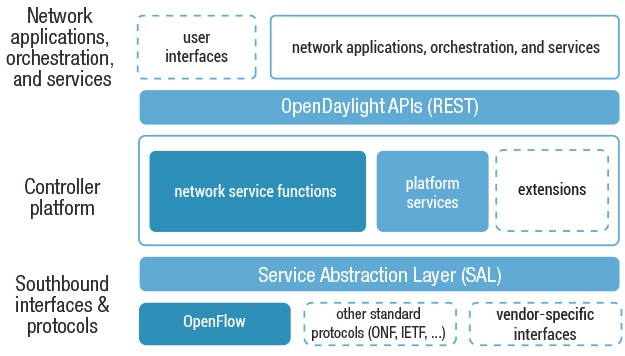
\includegraphics[width=10cm]{./includes/opendaylight.jpg}
	\caption{The proposed OpenDaylight architecture.}
	\label{fig:opendaylight}
\end{figure}
	
The momentum that \ac{sdn} is getting might be explained by a general need for change in the networking industry. Operators primarily want to get more control over their networks, something which using the current stack of protocols is relatively complicated to get. The original \acs{osi} reference model \cite{zimmermann} touches on the ``Management Aspects'' of each layer in the model, a way for management entities in the highest layer to control the behavior of lower layers. Unfortunately in the swift evolution of \ac{tcp}/\ac{ip}, these management interfaces are often limited or absent all together. 



	\subsection{Research Question} % (fold)
	\label{sub:research_question}
	It is unclear if a real-world OpenFlow and \ac{sdn} implementation will actually provide any simplicity, additional flexibility or cost savings when compared to contemporary technologies \cite{programmability-answer}. And so the question arises: \textsl{``How much can operators benefit from using OpenFlow when implementing \aclp{dvpn}?''} 
	This requires research into whether \acp{dvpn} can be provisioned by current technologies and how this can be implemented in the network. Additionally, we will research the possibility of implementing \acp{dvpn} using OpenFlow. And finally we will attempt to prove the hypothesis that OpenFlow will reduce the complexity in the architecture of the management systems and the network as a whole.

	% subsection research_question (end)

	\subsection{Scope} % (fold)
	\label{sub:scope}
	The focus will primarily be on deploying \acp{ppvpn} at Layer 2 of the \acs{osi}-model between end-users. We haven chosen to do so because these Ethernet \acp{vpn} are characterized by their transparency to the end-user, who will be placed in a single broadcast domain with its peers and can thus communicate directly without configuring any sort of routing.
	
	Previous research in \cite{net-prog-vpn} has proposed a very specific implementation for programmable networks to deploy on-demand \acp{vpn} but it predates the OpenFlow specification, and also omits a comparison with how this would look using contemporary technologies.

	% subsection scope (end)

	\subsection{Approach} % (fold)
	\label{sub:approach}
	In the Section~\ref{sec:dvpns} we will define the conceptual design of \acp{dvpn}. This will result in a list of required features for the technologies to provide such a service. Section~\ref{sec:implementation} will list the technologies available and will additionally determine their usability for implementing \acp{dvpn} when taking into account the requirements set forth in Section~\ref{sec:dvpns}. In Section~\ref{sec:results} we will distill the advantages and limitations of the different implementations and substantiate how the compare to each other. Finally, Section~\ref{sec:conclusion} summarizes the results and provides a discussion and future work on this subject.

	% subsection approach (end)

% section introduction (end)
		\clearpage
		
		% (c) 2014 Michiel Appelman
\section{State of the Art} % (fold)
\label{sec:state_of_the_art}

The issue of creating dynamic \acp{vpn} within \ac{sp} networks apparently comes from the inability to do so using technologies available to operators today. To get an understanding of how we got to this point and where the limitations or obstacles lie, an overview of the state of the art is required.

To be qualified to provide network operators with dynamic \acp{vpn} each technology will need to be able to provide the following features:

\begin{enumerate}
	\item scalable up to thousands of (dynamic) Layer 2 \acp{vpn} and client \acsp{mac},
	\item fast failover times (<50ms) to provide continuity to critical applications,
	\item efficient use of, and control over all network resources, and
	\item provide \acl{qos} features to differentiate between classes of applications. 
\end{enumerate}

\subsection{\acs{sdh}/\acs{sonet}} % (fold)
\label{sub:sdh_sonet}
The foundation of \acp{wan} today is still \ac{sdh} and its North-American counterpart \ac{sonet}. It operates at Layer 1 and is concerned with putting various data streams on fiber links. \ac{sdh} networks find their origin in the telecommunications world where it was developed to transfer real-time cell switched voice data. It quickly evolved to include \ac{atm} and later also Ethernet. Due to its maturity the protocol is considered stable but is also very static in its manageability. Developments are ongoing in the \ac{gmpls} field to bring dynamic configuration to \ac{sdh} devices, but they are in their infancy.

% subsection sdh_sonet (end)

\section{\acs{atm}} % (fold)
\label{sec:atm}
\ac{atm} is a legacy protocol that has been used by operators to carry traffic over the internet backbone since the 1990s. Where as Ethernet and \ac{ip} are developed as packet-routing connection-less protocols, \ac{atm} is a cell-switched connection-oriented protocol. This poses a number of problems when trying to transport \ac{ip} over \ac{atm}. First, the variable length of the packets don't map efficiently to the fixed size cells of \ac{atm}. Drops of a single cell would cause the entire frame to become unusable. Then there is the added overhead of encapsulating \ac{ip} over \ac{atm}, which causes inefficient use of the network resources when compared to running an all \ac{ip} network. Finally, the \ac{qos} features of \ac{atm} are left unused. These problems are some of the reasons that operators have moved away from \ac{atm} based backbones, to all \ac{ip} ones. 

As mentioned, \ac{atm} does provide \ac{qos} to the network operators which they used extensively. The protocol also allows for the granular control of network paths -- called circuits -- but at a price; management over an \ac{atm} network has to be tightly controlled for it to function properly. This limits its dynamism and scalability, which (also considering the aforementioned objections) does not make it a viable candidate to implement dynamic \acp{vpn}.

% section atm (end)

\subsection{\acs{mpls}} % (fold)
\label{sub:mpls}
\ac{mpls} is known for its scalability and extensibility. Over the past decade additions have been made to the original specification to overcome a plethora of issues within carrier networks. This initially started with trying to implement fast forwarding in legacy switches using labels (or tags) at the start of the frame \cite{tag-switching}. When this issue became surmountable using new hardware, \ac{mpls} had already proven to be capable of transporting a wide arrange of protocols on the carrier backbone network, all the while also providing scalability, \ac{te} and \ac{qos} features to the operators.

\ac{mpls} itself is more a way of forwarding frames through the network, without facilitating any topology discovery, route determination, resource management, etc. These functions are left to a stack of other protocols. To discover the topology, \ac{mpls} relies on an \ac{igp}. The distribution of labels is done using \ac{ldp} and/or \ac{rsvp}, of which the latter also provides granular \ac{te} and \ac{qos} functionalities.

\acp{vpn} are also provided by additional protocols. Layer 3 \acp{vpn} make use of \ac{bgp} to distribute client prefixes to the edges of the carrier network. The core is only concerned with the forwarding of labels and has now knowledge of these \acs{ip} prefixes. Layer 2 \acp{vpn} make use of \ac{ldp} and \ac{vpls}, a service which encapsulates the entire Ethernet frame and pushes a label to it to map it to a certain separated network. Again, the core is only concerned with the labels and only the edges need to know the clients \acs{mac} addresses. 

Because of its extensibility the \ac{mpls} technology and the added protocols and tools, it is commonly used in \acp{cen} as an alternative to legacy \acs{atm} and \acs{sdh} networks. With added features such as \ac{ecmp}, \ac{frr} and explicit routing it has proven to be a technology fit for carriers to transport critical applicition traffic over large networks. \ac{mpls} thus meets the requirements set forth, which might be the reason for its widespread use presently. However, given the scale and criticality of the networks and the stack of various protocols to implement it, management of \ac{mpls} networks has remained fairly static and mostly a manual task.

% subsection mpls (end)

\subsection{\acs{spb}} % (fold)
\label{sub:spb}
\ac{spb} is an evolution of the original \acs{ieee} 802.1Q \ac{vlan} standard. \ac{vlan} tags have been in use in the networking world for a long time and provide decent separation in campus networks. However, when \ac{vlan}-tagging was done at the customer network, the carrier couldn't separate the traffic from different customers anymore. This resulted in 802.1Qad or Q-in-Q which added an S-\ac{vlan} tag to separate the client \acp{vlan} from the \ac{sp} \acp{vlan} in the backbone. This was usable for the Metro Ethernet networks for awhile but when \acp{sp} started providing this services to more and more customers, their backbone switches could not keep up with the clients \ac{mac} addresses.

To solve this scalability problem \ac{pbb} (802.1Qay or \ac{mac}-in-\ac{mac}) was introduced. It encapsulates the whole Ethernet frame on the edge of the carrier network and forwards the frame based on the Backbone-\ac{mac}, Backbone-\ac{vlan} and the I-SID. The I-SID is a Service Instance Identifier, which with 24 bits is able to supply the carrier with 16 million separate networks. The downside of \ac{pbb} remained one that is common to all Layer 2 forwarding protocols: the possibility of loops. Preventing them requires \ac{stp} which will disable links to get a loop-free network. Disadvantages of \ac{stp} include the relatively long convergence time and inefficient use of resources due to the disabled links. This final problem was solved by using \acs{isis} as a routing protocol to distributed the topology and creating \acp{spt} originating from each edge device. This is called \ac{spb} or 802.1aq.

\ac{spb} benefits from the maturity of the Ethernet protocol by reusing protocols for \ac{oam} and \ac{pm} and the fact that only the edges of the network need to be \ac{spb} capable -- the core switches just need to be able to forward 802.1Qad frames. Manageability of \ac{spb} \acp{vpn} is simplified to mapping a certain customer port or \ac{vlan} to an I-SID. Limitations of \ac{spb} include a very coarse way to apply \ac{te} policies or \ac{ecmp} load sharing. Although drafts are in the works to resolve this limitation, this has yet to be standardized and implemented. Finally, the protocol at this point lacks fast failovers, and as such will not be a viable option to implement dynamic \acp{vpn}.


% subsection spb (end)

\subsection{\acs{trill}} % (fold)
\label{sub:trill}
There has been discussion going on between \ac{spb} and \ac{trill} supporters as to which is the `better' protocol. Indeed, both use \ac{isis} as an \ac{igp} and both try to solve the same problem to make Ethernet networks scalable to the desired scale of networks in use today, but they differ in their premise and implementation. \ac{trill} adds a completely new header on top of  the Ethernet frame with a source and destination RBridge allowing the so-called RBridges to route -- Layer 3 -- the frame to its destination over the \ac{trill} backbone network.

Without this paper turning into another \ac{trill} versus \ac{spb} comparison, it is important to point out various differences in the two technologies with regards to our proposed use-case. First, the hop-by-hop decision making by \ac{trill} has the benefit of being able to distribute traffic in more efficient way over a dense network. \ac{spb} on the other hand makes its forwarding decision at the head-end, similar to \ac{mpls} forwarding. This means that careful consideration needs to take place to choose either more efficient \ac{ecmp} forwarding or granular control over forwarding paths. 

Additionally, because \ac{trill} is a completely new protocol, the \ac{ietf} is also still working on adding some essential features that are still in draft. These include \ac{qos}, \ac{oam}, \ac{pm} and \ac{te}. And finally there is another limitation for \acp{cen}, which is the lack of network separation. \ac{trill} only supports the 4096 \ac{vlan} tags present in the 802.1Q frame to separate customer networks. At this point, it will fail to meet the requirements to provide dynamic \acp{vpn}.

% subsection trill (end)





\subsection{OpenFlow} % (fold)
\label{sub:openflow}
What is it? Relation to \ac{sdn}.

The momentum comes from a general problem with control over the network (Zimmerman OSI)

Also, ATM style controls.



% subsection openflow (end)

% section state_of_the_art (end)		
		\clearpage
		
		% (c) 2014 Michiel Appelman
\section{Design} % (fold)
\label{sec:design}

\subsection{Requirements} % (fold)
\label{sub:requirements}
\begin{enumerate}
	\item What will the system need to look like?
	\item What are its functional requirements?
	\item What is the input?
	\item What is the expected output?
	\item How can it be extended in a later stage?
\end{enumerate}

To further shape the actual design of the system, we will specify what this \ac{dvpn} service will need to look like. 

First, we will need to define a certain input. Our design accepts a set of physical ports with an optional C-\ac{vlan} corresponding to it. This set represents the group of users which will be placed in a single \ac{vpn} and thereby connected to each other. It also requires the values for minimum and maximum bandwidth used by \ac{dvpn} over the network. High bandwidth \acp{dvpn} may need load-sharing over multiple physical 1GbE links for example.

Second, the output will be defined as the \ac{vpn} created throughout the network and Layer 2 connectivity between the chosen endpoints from the input.

Third, the usage of the network resources should be monitored during the lifetime of the \ac{dvpn}. If certain links are nearing their capacity, \acp{dvpn} should be able to move paths to links where more resources are available.

Finally, the tearing down of the \ac{dvpn} will also need to be arranged so as to free up resources for new \acp{dvpn}.

A design for the complete process will be given in the following sections, first in a situation where traditional network management and \ac{mpls} are used. And after that using the \ac{sdn} approach and its way of managing network devices.

% subsection requirements (end)

\subsection{\acs{mpls}} % (fold)
\label{sub:contemporary}
To start:
\begin{enumerate}
	\item Input goes where?
	\item Flow of information.
	\item Amount and type of output.
\end{enumerate}

As has been discussed in Section~\ref{sub:mpls} a typical \ac{mpls} network consists of a stack of routing protocols. This means that to provision the \ac{dvpn} several protocols will be affected. 

First, determine best path and configure \ac{rsvp} to make paths between \acp{pe}. Needs \ac{te} input. 

Second, \ac{vpls} to add the ports to the \ac{vpls} instance and define the paths to use.

Check before enabling: 
\ac{rsvp} for state of tunnel between \acp{pe} and
\ac{ldp} for adjacency between \ac{vpls} instances on \acp{pe}

Monitor utilization of links and when links become full, move paths over them to different paths. This can be done by periodically getting interface statistics from the network devices through \ac{snmp} or sFlow. The \ac{nms} will need to store the links that a path is taking when the \ac{dvpn} is set up, so the correct paths may be adjusted to move traffic away. The decision on when to do so depends on the service level of the carrier, who for example may allow for a certain amount of oversubscription. To prevent the algorithm from constantly moving paths between different links it is also recommended to apply some kind of timing mechanism.

To minimize traffic impact when moving a path in use by a \ac{dvpn} to another set of links the \ac{rsvp} \ac{frr} option can be used to add a backup path to the \ac{vpls} instance. If a backup path already exists, it will be replaced. As soon as the new path is installed, the traffic of the \ac{dvpn} can be migrated to the backup path. This path will then be set as the primary path and the previous backup path can be reinstalled. This process will require additions in the \ac{rsvp} paths and addition to the \ac{vpls} instance. The path should be checked for 

In the access layer, \ac{mpls} has to be supported. Otherwise no mapping to customer \ac{vlan}, only per port. Other option: Q-in-Q but mapping of C AND S-TAG to VPLS instance needs to be supported by \ac{pe}.

% subsection contemporary (end)

\subsection{OpenFlow} % (fold)
\label{sub:openflow}
To start:
\begin{enumerate}
	\item Input goes where?
	\item Flow of information.
	\item Amount and type of output.
\end{enumerate}

Use \ac{mpls} labels to tag traffic for separate \acp{dvpn}. If running a label distribution protocol on controller, \ac{p}-routers might even be \ac{mpls}-only.

Need OpenFlow support on access-layer, or Q-in-Q to map to MPLS tag at \ac{pe}, OR match on \ac{mac}.



% subsection openflow (end)



% section design (end)
				
		\clearpage
		
		% (c) 2014 Michiel Appelman
\section{Results} % (fold)
\label{sec:results}

The features and limitations of the three discussed technologies in Section~\ref{sec:implementation} are given in Table~\ref{tb:reqs}. In this section we will compare the contemporary technologies with the OpenFlow implementation when implementing the \ac{dvpn} service as discribed in Section~\ref{sec:dvpns}.

\begin{table}[h]
	\centering
	\begin{tabular}{r|lll}
	 & \acs{spb} & \acs{mpls} & OpenFlow / \acs{sdn}\\
	\hline
	Tagging of VPN Traffic & \acs{pbb} & \acs{vpls} (\acs{mpls}) & \acs{pbb} / \acs{mpls}\\
	MAC Scalability & yes & yes & yes\\
	Topology Discovery & \acs{isis} & \acs{ospf} & application\\
	Path Provisioning & \acs{spt} & \acs{rsvp} / \acs{ldp} & application\\
	Traffic Engineering & limited & \acs{rsvp} & application\\
	\ac{ecmp} & limited & yes & yes, using Groups\\
	\ac{bum} limiting & dependent on \acs{hw} & dependent on \acs{hw} & yes, using Metering\\
	Exchange \acsp{cmac} & no & \ac{evpn} (draft) & application\\
	Ingress Rate Limiting & dependent on \acs{hw} & dependent on \acs{hw} & yes, using Queues or Metering\\
	Fast Failover & no & \acs{frr} & yes, using Groups\\
	\acs{oam} & 802.1ag / Y.1731 & \acs{lsp} Ping / \acs{bfd} & application\\
	\hline
	Forwarding Decision & \acs{pbb} tags & \acs{mpls} labels & flow entry \\
	\ac{bum} traffic handling & flood & flood & sent to controller\\
	\end{tabular}
	\caption{Feature requirements available in discussed technologies.}
	\label{tb:reqs}
\end{table}


\subsection{\acs{spb}} % (fold)
\label{sub:r-spb}

The \ac{spb} architecture allows for a scalable carrier network supporting thousands, even millions of \acp{dvpn} using the \ac{isid} in the \ac{pbb} frame. From our theoretical implementation in Section~\ref{ssub:spb}, it became evident that setting up a \acp{dvpn} requires little configuration. The \ac{isid} only needs to be configured on the \ac{pe} connecting the \ac{ce} port and the \ac{isis} routing protocol distributes this binding to the other corresponding \acp{pe}. Another benefit is the use of Ethernet \ac{oam} standards that are mature and extensive to allow for precise monitoring and troubleshooting.

However, the simplicity of the architecture comes at a cost. The protocols has:
\begin{itemize}
	\item limited explicit or constraints-based routing, meaning few \ac{te} features,
	\item limited \ac{ecmp} functionality due to the infancy of the standard to support it, and
	\item because, failure recovery depends on \ac{isis} reconvergence, no fast failover.
\end{itemize}

These limitations are being worked on by the community, e.g.\ IEEE 802.1Qbp which provides extensive \ac{ecmp} functions. And since the technology has only been officially standardized since March 2012, it will also need to mature before it is suitable for carrier implementations.  

Because of the shortcomings of \ac{spb} with regards to the use-case set forth in Section~\ref{sec:dvpns}, we will omit this technology in our comparison. Instead we will focus on comparing the \ac{mpls} setup from Section~\ref{ssub:mpls} with the \acs{sdn}/OpenFlow architecture as designed in Section~\ref{sub:openflow}.

% subsection r-spb (end)

\subsection{Comparison} % (fold)
\label{sub:comparison}

To get an overview of the key differences between the two architectures we will follow the structure of the \ac{dvpn} requirement list defined in Section~\ref{sec:dvpns}. 

\subsubsection{Service} % (fold)
\label{ssub:service}

From a customer point-of-view it should be of no concern how the \ac{dvpn} service is implemented in the provider network. Moreover, the \acp{pe} and the rest of provider network should be completely transparent. As such, the two technologies do not show any difference in their implementation. Both technologies are able to 
\begin{inparaenum}[\itshape 1\upshape)]
	\item provide a Layer 2 broadcast domain,
	\item connect \acp{ce} without any required \ac{vpn} configuration on them, and
	\item be completely transparent to the \acp{ce}.
\end{inparaenum}

% subsubsection service (end)

\subsubsection{Transport} % (fold)
\label{ssub:transport}

Both implementations use \ac{mpls} labels to transport frames through the network. By using labels to identify and route traffic over paths instead of a hop-by-hop based routing protocol that uses an egress \ac{pe} identifier, both technologies allow for granular \ac{te} features.   The usage of paths also means that the \acp{p} will forward the traffic without relying on or being aware of any \acp{cmac}, providing scalability. OpenFlow supports \ac{mpls} labels since version 1.1. Version 1.0 can only separate traffic using C-\ac{vlan} tags, which means that 
\begin{inparaenum}[\itshape a\upshape)]
	\item the customer \acp{mac} will need to be present in the backbone, 
	\item the customer can not use \acp{vlan} over the provider network, and
	\item forwarding will be based on the egress \ac{pe}, not the path, eliminating \ac{te}.
\end{inparaenum}
This latter limitation can of course be overcome using more specific match entries for every traffic flow that needs to be forwarded in certain way, however this would negate the benefit of using \ac{mpls} labels to minimize the amount of flows needed in the backbone. These specific flows are called `microflows' and while giving more precise control over traffic, they will fill up the flow tables of \acp{p} fairly quickly in a provider network with thousands of customers. The only way for OpenFlow to scale up to a carrier network level is by using version 1.1 or later.

Comparing \ac{mpls} to the \ac{vc}-based \ac{atm} protocol which required configuration of \acp{vc} throughout the network, we find that \ac{mpls} has the benefit of automatically distributing labels which allows for scalable and easily configurable carrier networks. The \acp{lsp} in \ac{mpls} are very comparable to the \acp{vc} of \ac{atm} \cite{mpls-tunnels}. Managing and configuring \acp{vc} was a problem in the \ac{atm} days though, mainly because of the lack of integration between the \ac{atm} switches and \ac{ip} routers. So \ac{ldp} was a huge advantage in the eyes of the carriers in the early days of \ac{mpls}. However, with the advent of explicit routes using \ac{rsvp} for \acl{te}, operators are now trying to do away with the automatic paths setup by \ac{ldp}. With these strict forwarding controls they are but a small step removed from once again manually setting up \acp{vc}. 

As mentioned before, OpenFlow will also need to provide path-based forwarding to provide scalability in the network and this has to be implemented with strict control over the labels in each \ac{pe} and \ac{p}. However, the advantage that operators have today is that the complete control plane of the network will be in the OpenFlow controller and its applications. The \ac{atm} setup required separate management for the \ac{atm} switches and the \ac{ip} routing subsystems such as the \ac{igp} and \ac{bgp} with limited integration between the two.

A prerequisite for providing any kind of service over a network is the knowledge of the network topology. Again the distinction between decentralized and centralized is easily made. Arguments can be made about the faster convergence of large networks using a centralized controller, however these claims are largely dependent on the implementation. Transporting frames any of the two technologies will not change depending on the implementation chosen. We will however take a look at how they differ in provisioning procedures in the Section~\ref{ssub:provisioning}.

OpenFlow has been able to provide \ac{ecmp} since version 1.1 using Groups with the \textbf{select} type. It basically means that a flow can point to this group and it will choose one of the output ports, based on a hashing algorithm. And although the terminology is different from Link Aggregation Groups, the procedure is indeed the same. Moreover, due to the lack of a definition for the hashing algorithm, both implementations depend on the hashing algorithm implemented by the vendor to provide efficient load sharing.

In a contemporary setup devices support fast failover by setting up \ac{bfd} sessions between each other to monitor liveness of the path. This is done within the forwarding plane of the device and with very small timeouts so failures will be apparent within milliseconds. Currently OpenFlow devices lack the ability to install some sort of packet generator in the forwarding plane to perform the same functionality. \ac{sdn} researchers have proposed to use a monitoring function closer to the data plane in \cite{scalable-fault} but until that has been implemented monitoring of paths will need to use the controller, causing higher recovery times. Monitoring of individual physical links is possible and using the \textbf{fast failover} Group type though. This allows the network device to quickly reroute without needing to consult the controller.

Rate Limiting

MAC learning in control in draft E-VPN


% subsubsection transport (end)

\subsubsection{Provisioning} % (fold)
\label{ssub:provisioning}

Discovering the network topology of a distributed network requires connectivity between the devices on Layer 2 or 3 (depending on the \ac{igp}) before any information can be exchanged. This means setting up a network to provide \acp{dvpn} will require some up-front configuration from the \ac{nms} as well. Using OpenFlow on the other hand, the only requirement is setting up a connection to the controller from all networking devices. 

\acl{te} can benefit from centralization as well. In fact, operators already need to store information on application traffic flows and requirements in the \ac{nms} when using \ac{mpls} to route traffic in a certain way. When using \ac{rsvp} with explicit routes, the \ac{nms} requires a complete view from the network to correctly define paths. Only when using loose constraints, the \ac{te} functionality is partly solved decentralized using \ac{cspf}. However, the \ac{nms} still needs to configure the constraints for each flow. An \ac{sdn} setup provides the operator with a complete view from the network as seen by the controller which can be used together with input from \ac{dvpn} constraints to optimize the paths. The advantage lies in the fact that the the \ac{te} application on the controller can get the current topology directly from the discovery application. Whereas the \ac{mpls} setup would require the \ac{nms} to retrieve the topology from the network, or the topology should be predefined. Either way, this might lead to inconsistencies, depending on the implementation.


MPLS:
\begin{itemize}
	\item initial setup complicated
	\item DVPN setup: only each PE with member port
	\item 
\end{itemize}

OF:
\begin{itemize}
	\item initial setup nonexistent, no VPNs = no flows (except LLDP/OAM)
	\item DVPN setup: every PE with member port + Ps in path
	\item 1.0 supported almost everywhere, 1.1 and 1.2 are not. 1.3 slowly coming. 
	\item TE more intricate algorithms on faster hardware (knapsack problem)
\end{itemize}

1.3 Controllers:
Ryu by NTT \cite{ryu}
NOX extensions by CPqD research center from Brasil \cite{cpqd}
M\"{u}L from kulcloud (South-Korea) is coming \cite{mul}

OpenDaylight controller still lacks 1.3 support

\HRule

The strength of these applications however, is the fact that operators can integrate their \ac{nms} and control plane even more. This allows for a more granular control over their traffic.

MPLS automation software written for DVPNs, but not due to lack of programmable consistent interface to HW, not portable to other vendor, sometimes even model!

complexity high due to intricate dependencies of different protocols

\HRule

OF applications need to solve from ground up, topology, etc... nortbound interface undefined, limited portability of apps between controllers. 


\ac{mpls} \acp{vpn} in OpenFlow: \cite{mpls-vpn-openflow}

\ac{mpls} control plane in OpenFlow: \cite{mpls-open}

Also: access layer intelligence.


% subsubsection provisioning (end)





% subsection comparison (end)





% section results (end)				
		\clearpage
		
		% (c) 2014 Michiel Appelman
\section{Conclusion} % (fold)
\label{sec:conclusion}

% section conclusion (end)

\section{Future Work} % (fold)
\label{sec:future_work}

Other use cases:
\begin{itemize}
	\item multi-domain
	\item mobility
	\item smart metering
\end{itemize}

% section future_work (end)				
		\clearpage
		
	%%%%%%%%%%%%%%%%%%%%%%%%%%%
	%%      Appendices       %%
	%%%%%%%%%%%%%%%%%%%%%%%%%%%
		\appendix
		\noappendicestocpagenum
		\addappheadtotoc
		\pagestyle{fancy}
		\renewcommand{\sectionmark}[1]{% 
		\markboth{#1}{}}
		\fancyhead[L]{\small{\nouppercase{\leftmark}}}
		\fancyhead[R]{\nouppercase{\emph{\appendixname\ \LARGE{\thesection}}}}
		\renewcommand{\headrulewidth}{0.5pt}

	%%%%%%%%%%%%%%%%%%%%%%%%%%%
	%%%%%%%%%%%%%%%%%%%%%%%%%%%
		% Acronyms
		% (c) 2014 Michiel Appelman
\twocolumn
\section{Acronyms}
\begin{acronym}[AMS-IX]
%	\acro{}[\acrstyle{}]{\expstyle{}}
	\acro{api}[\acrstyle{api}]{\expstyle{Application Programming Interface}}
	\acro{arp}[\acrstyle{arp}]{\expstyle{Address Resolution Protocol}}
	\acro{atm}[\acrstyle{atm}]{\expstyle{Asynchronous Transport Method}}
	\acro{bfd}[\acrstyle{bfd}]{\expstyle{Bidirectional Forward Detection}}
	\acro{bgp}[\acrstyle{bgp}]{\expstyle{Border Gateway Protocol}}
	\acro{bum}[\acrstyle{bum}]{\expstyle{Broadcast, Unknown unicast and Multicast}}
	\acro{ce}[\acrstyle{ce}]{\expstyle{Customer Edge device}}
	\acro{cen}[\acrstyle{cen}]{\expstyle{Carrier Ethernet Network}}
	\acro{cmac}[\acrstyle{c-mac}]{\expstyle{Customer \acs{mac}}}
	\acro{cots}[\acrstyle{cots}]{\expstyle{Commercial Off-The-Shelf}}
	\acro{cpu}[\acrstyle{cpu}]{\expstyle{Central Processing Unit}}
	\acro{cspf}[\acrstyle{cspf}]{\expstyle{Constrained Shortest Path First}}
	\acro{da}[\acrstyle{da}]{\expstyle{Destination Address}}
	\acro{dos}[DoS]{\expstyle{Denial of Service}}
	\acro{dvpn}[DVPN]{\expstyle{Dynamic \acs{vpn}}}
	\acro{ecmp}[\acrstyle{ecmp}]{\expstyle{Equal Cost Multi Path}}
	\acro{ect}[\acrstyle{ect}]{\expstyle{Equal Cost Trees}}
	\acro{evpn}[\acrstyle{e-vpn}]{\expstyle{Ethernet \acs{vpn}}}
	\acro{fcs}[\acrstyle{fcs}]{\expstyle{Frame Check Sequence}}
	\acro{fpga}[\acrstyle{fpga}]{\expstyle{Field Programmable Gate Array}}
	\acro{frr}[\acrstyle{frr}]{\expstyle{Fast Reroute}}
	\acro{gmpls}[\acrstyle{gmpls}]{\expstyle{Generalized \acs{mpls}}}
	\acro{hw}[\acrstyle{hw}]{\expstyle{Hardware}}
	\acro{icmp}[\acrstyle{icmp}]{\expstyle{Internet Control Message Protocol}}
	\acro{ieee}[\acrstyle{ieee}]{\expstyle{Institute of Electrical and Electronics Engineers}}
	\acro{ietf}[\acrstyle{ietf}]{\expstyle{Internet Engineering Task Force}}
	\acro{igp}[\acrstyle{igp}]{\expstyle{Interior Gateway Protocol}}
	\acro{io}[\acrstyle{io}]{\expstyle{Input/Output}}
	\acro{ip}[\acrstyle{ip}]{\expstyle{Internet Protocol}}
	\acro{isis}[\acrstyle{is-is}]{\expstyle{Intermediate System-Intermediate System}}
	\acro{itut}[\acrstyle{itu-t}]{\expstyle{International Telecommunication Union - Technology}}
	\acro{lan}[\acrstyle{lan}]{\expstyle{Local Area Network}}
	\acro{ldp}[\acrstyle{ldp}]{\expstyle{Label Distribution Protocol}}
	\acro{lsp}[\acrstyle{lsp}]{\expstyle{Label-switched Path}}
	\acro{mac}[\acrstyle{mac}]{\expstyle{Media Access Control}}
	\acro{mef}[\acrstyle{mef}]{\expstyle{Metro Ethernet Forum}}
	\acro{mpls}[\acrstyle{mpls}]{\expstyle{Multi Protocol Label Switching}}
	\acro{nms}[\acrstyle{nms}]{\expstyle{Network Management System}}
	\acro{oam}[\acrstyle{oam}]{\expstyle{Operations, Administration and Management}}
	\acro{oflops}[\acrstyle{oflops}]{\expstyle{OpenFlow Operations Per Second}}
	\acro{onf}[\acrstyle{onf}]{\expstyle{Open Networking Foundation}}
	\acro{osi}[\acrstyle{osi}]{\expstyle{Open System Interconnect}}
	\acro{ospf}[\acrstyle{ospf}]{\expstyle{Open Shortest Path First}}
	\acro{os}[\acrstyle{os}]{\expstyle{Operating System}}
	\acro{pbb}[\acrstyle{pbb}]{\expstyle{Provider Backbone Bridging}}
	\acro{pci}[\acrstyle{pci}]{\expstyle{Peripheral Component Interconnect}}
	\acro{p}[\acrstyle{p}]{\expstyle{Provider device}}
	\acro{pe}[\acrstyle{pe}]{\expstyle{Provider Edge device}}
	\acro{pm}[\acrstyle{pm}]{\expstyle{Performance Measurement}}
	\acro{ppvpn}[\acrstyle{ppvpn}]{\expstyle{Provider-provisioned \acs{vpn}}}
	\acro{qos}[QoS]{\expstyle{Quality of Service}}
	\acro{ram}[\acrstyle{ram}]{\expstyle{Random Access Memory}}
	\acro{rsvp}[\acrstyle{rsvp}]{\expstyle{Resource Reservation Protocol}}
	\acro{sa}[\acrstyle{sa}]{\expstyle{Source Address}}
	\acro{sdh}[\acrstyle{sdh}]{\expstyle{Synchronous Digital Hierarchy}}
	\acro{sdn}[\acrstyle{sdn}]{\expstyle{Software Defined Networkinging}}
	\acro{sonet}[\acrstyle{sonet}]{\expstyle{Synchronous Optical Network}}
	\acro{spb}[\acrstyle{spb}]{\expstyle{Shortest Path Bridging}}
	\acro{spt}[\acrstyle{spt}]{\expstyle{Shortest Path Tree}}
	\acro{sp}[\acrstyle{sp}]{\expstyle{Service Provider}}
	\acro{sram}[\acrstyle{sram}]{\expstyle{Static \acs{ram}}}
	\acro{stp}[\acrstyle{stp}]{\expstyle{Spanning Tree Protocol}}
	\acro{tcam}[\acrstyle{tcam}]{\expstyle{Ternary Content-Addressable Memory}}
	\acro{tcp}[\acrstyle{tcp}]{\expstyle{Transmission Control Protocol}}
	\acro{te}[\acrstyle{te}]{\expstyle{Traffic Engineering}}
	\acro{tor}[ToR]{\expstyle{Top of Rack}}
	\acro{tos}[\acrstyle{tos}]{\expstyle{Type Of Service}}
	\acro{trill}[\acrstyle{trill}]{\expstyle{Transparent Interconnection of Lots of Links}}
	\acro{udp}[\acrstyle{udp}]{\expstyle{User Datagram Protocol}}
	\acro{vc}[\acrstyle{vc}]{\expstyle{Virtual Circuit}}
	\acro{vlan}[\acrstyle{vlan}]{\expstyle{Virtual \acs{lan}}}
	\acro{vpls}[\acrstyle{vpls}]{\expstyle{Virtual Private \acs{lan} Service}}
	\acro{vpn}[\acrstyle{vpn}]{\expstyle{Virtual Private Network}}
	\acro{wan}[\acrstyle{wan}]{\expstyle{Wide Area Network}}

\end{acronym}
\onecolumn


		\clearpage

		% Bibliography
		\renewcommand*{\refname}{} % This will define heading of bibliography to be empty, so you can...
		\section{Bibliography}
		\bibliographystyle{ieeetr}
		\bibliography{data/bibliography}

	%%%%%%%%%%%%%%%%%%%%%%%%%%%
	%%%%%%%%%%%%%%%%%%%%%%%%%%%
		% Acknowledgements
		\clearpage
		\pagestyle{empty}
		\hfill \\[6cm]
		\section*{Acknowledgements}
		\textsl{Thanks to Rudolf Strijkers for his supervision during this project.}
\end{document}